\section{System Overview}


This paper describe our system for bimanual sewing with a curved needle. We use two robots to manipulate the needle, i.e. piercing and pass from one robot to another. Two KUKA robots are mounted with needle drivers to grip the needle. In addition to these, a third robot is used to control the fabric tube. An special mandrel is designed to support the fabric tube and bound it tightly with the stent. Holes on the mandrel allow the needle to go through and hence stitch the stent and the fabric together. Our sewing task requires high accuracy and robustness. Each stitch is required to be at the exact place and have the same length. We use a vision system to guide the robot movements in order to maintain the accuracy. The needle position is tracked during the whole task. The robot movements are computed online to deliver the needle to stitch at the correct spot. The robot movements are programmed by human demonstrations.

We adopt an bimanual sewing approach: the curved needle is first carried by one robot (A) to pierce the fabric, and picked up by another robot (B) from the other side. The needle is then pulled out by the robot B and passed back to the robot A. The third robot moves to the next stitch position. These movements complete one cycle and repeat the cycle until the whole stent is sewed.



\subsection{Hardware setup}

%------------- Curved needle  --------------
\begin{figure}
\centering
{
\subfloat[\scriptsize{Curved needle}] {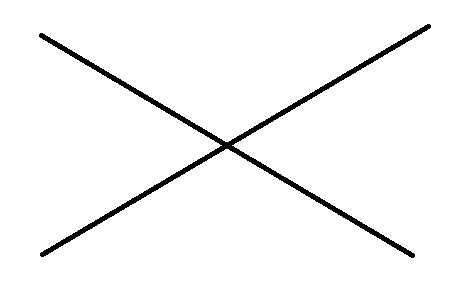
\includegraphics[width=3cm]{./fig/void.jpg}}
\subfloat[\scriptsize{Needle driver griping needle}]  {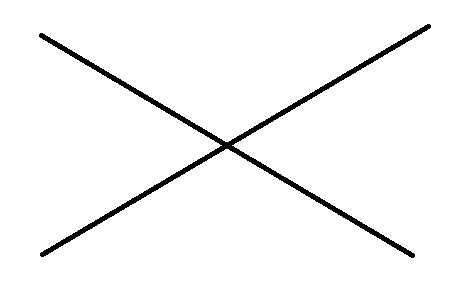
\includegraphics[width=3cm]{./fig/void.jpg}}
\caption{\scriptsize{Curved needle}}
\label{fig:curvedneedle}
}
\end{figure}
%------------- Needle driver  --------------

The motorized needle driver mounted on the robot is shown as Fig.1. This device incorporates a medical used Mayo Hager needle driver. This needle driver is widely used in laparoscopic surgery, the design of which can hold firming a surgical curved needle. The needle driver is motorized for robot to drive it. The design projective is that the needle driver can be controlled without mounting a motor directly on its rotation axis, which may impede the needle driver approaching the sewn object in some direction. This design features two set of constraints/guiding slots working in conjunction with pins. The linear slot lies in the direction along the handle of the needle driver and the constraint slot is coaxial with the needle driver axis; therefore the motor rotation can be mapped to the open and close of the needle driver. To reduce frictions in driving this mechanism, bears are used. One feature of this design is that the two jaws of the needle driver work in an unsynchronized way. In the situation that the needle driver is not fully open, the center line of the grasper is located near one jaw which may create difficulty in approaching a target point and grasp precisely. One method to solve this disadvantage is to replace the linear guiding slot with slot with a critical geometry.

\subsection{Vision System}
As mentioned above, the needle is manipulate between two robots. During the sewing task, defect can easily occur by the slip between the needle and the needle drivers. This usually happen during the passing stage: when one robot pass the needle to another, small displacement of the optimal relative pose between the needle and the needle driver can occur. We use a stereo vision system to monitor the process and measure the displacements. Adaptive robot movements are then generated to compromise these small displacements and deliver the needle to the correct spot.

Needle tracking / re-detection

\subsection{Learning from human demonstration}
Hand sewing is an delicate task and programming the robot to do sewing task is time-stacking. We adopt an learning for human demonstration approach for this task. Our learning starts by demonstrating to the robot multiple times how to make a stitch. A $Gaussian Mixture Model$ (GMM)~\cite{cohn1996active} is used to encode the sewing motion and the generalised motion is then retrieved via $Gaussian Mixture Regression$ (GMR). Generally speaking, this learning process involves three phases:

\begin{enumerate}
\item{1}: Human demonstrate sewing skill
\item{2}: Motion segmentation
\item{3}: Primitive motions learning
\end{enumerate}

\subsubsection{Human demonstrate how to sew stent graft}
The first step is to recode the stitching motion from human demonstration. Human single side hand sewing motion is composed of a few stages: 1)approaching fabric, 2)piercing, 3)releasing needle, 4)griping the needle tip and 5)pulling the needle out, 6)passing the needle to another hand and 7)picking up the needle head. At the beginning of the task, the needle driver grip firming the needle hand. When the tip of the curved needle pierces out from the bottom of the fabric, the needle driver release the needle. The needle is remained in the same pose by the friction of the fabric. The needle driver is then approach the other end of the needle: the tip, and grip the tip. The needle is hence connected with the needle driver again and being pulled out from the fabric. Once the needle is completely pulled out from the fabric, the needle driver pass it to another driver to re-grip the needle head. A full circle of one stitch is hence done and it is ready to start the next stitch.

We use the kinesthetic teaching method to demonstrate all these stages to the robot. The robot is put in gravity compensation mode and its movement is guided by human. The needle driver open and close is controlled an electronic footpedal. The movement of the robot, as well as the needle driver status, i.e. open and close, are recorded. During the demonstration, when the needle driver is close, we assume the needle is firmly connected with the driver and hence no displacement between the needle and the driver will occur. Hence, during the demonstrations, we presume the relative pose between the needle and the driver is a constant value (Figure~\ref{fig:curvedneedle}).

% Object centric approach -----------------------------
We programme the robot in a learning manner and adopt an object centric approach. In the object centric viewpoint, the centre of an manipulation task the is object movement, i.e. the needle movement. In our task, the needle movements for each stitch should the exactly the same so that the quality of the sewing is maintained.

% Data format -----------------------------------------
All the trajectories are recorded in 6 d.o.f with euler angles $\{\alpha, \beta, \theta\}$ representation of the orientation and $\{x, y, z\}$ representing the robot end effector position.


\subsubsection{Motion segmentation}
With all the collected training data (sewing trajectories), we segment each trajectory to reflect the different stages of sewing and learn each stage independently. This segmentation is done based on the relation between the needle and its driver: attached or detached. When the needle is attached to the driver, we take the object centric approach and learn the needle movement so that the needle can repeat the same movement every time. When the needle is detach to the driver, we focus on learning the needle driver trajectory in order to reach the proper location to grip the needle. 

Therefore, we use the needle driver open and close events to segment the trajectories (Figure~\ref{fig:segment}). Each segment is then learned as a primitive movement and encoded by a statistical model.

%% DTW --------------------------------------
Before learning models for each primitive movements, we apply the Dynamic Time Warping (DTW)~\ref{berndt1994using} to align the data across different demonstrations. DTW is a technique that temporally warps the data and find the best match between two time series according to their key features (Figure~\ref{fig:dtw}). In our task, velocity variations do not effect the task quality and hence DTW does not effect our training data.

\begin{figure}
\centering
{
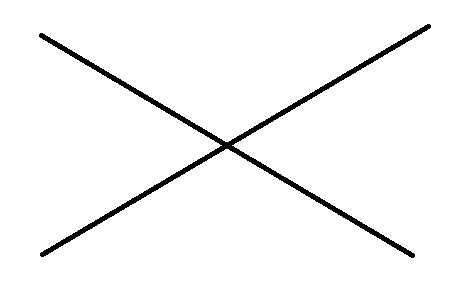
\includegraphics[width=3cm]{./fig/void.jpg}
\label{fig:dtw}
}
\end{figure}

\subsubsection{Primitive motion learning}

% GMM -------------------------------------------
After the we segments the data to a set of primitive movements, we build a model $Omega$ to encode each primitive. The same primitive of different trails of the demonstrations are put together as the training data. Each primitive is represented in seven dimension: one temporal value $\{t\}$, three spatial values $h=\{x, y, z\}$ and three orientation values $o=\{\alpha, \beta, \theta\}$. A joint distribution $p\{t,h,o\mid\Omega\}$ is builded by using $GMM$. We choose to use $GMM$ because of it's capability of encoding non-linear data and it's robustness of extracting constrains from noise data.

With $N$ Gaussian components, the joint distribution is represented as:

\begin{equation}
\begin{split}
p\left(t,h,o\mid\Omega\right) = \sum_{n=1}^N \pi_n p\left(t,h,o\mid\mu_n,\Sigma_n\right) \\
= \sum_{n=1}^N \pi_n \frac{1}{\sqrt{\left(2\pi\right)^D \mid\Sigma_n\mid }} e^{-\frac{1}{2}\left(\{t,h,o\}-\mu_n\right)^{\top} \Sigma^{-1}_n \left(\{t,h,o\}-\mu_n\right)}
\end{split}
\end{equation}
where $\pi_n$ is the prior of the $n^{th}$ Gaussian component, $D$ the number of variables,
and the ${\mu}_n$, ${\Sigma}_n$ the corresponding mean and covariance. For the $n^{th}$ Gaussian component, the mean and covariance $\mu_n$, $\Sigma_n$ is:

\begin{equation}
{
\boldsymbol{\mu}_n = \begin{pmatrix}    \boldsymbol{\mu}_{t,n}     \\
                                        \boldsymbol{\mu}_{h,n}          \\
                                        \boldsymbol{\mu}_{o,n}
                    \end{pmatrix}
\hspace{0.2in}
\boldsymbol{\Sigma}_n = \begin{pmatrix}     \boldsymbol{\Sigma}_{tt,n}  & \boldsymbol{\Sigma}_{th,n} & \boldsymbol{\Sigma}_{to,n}  \\
                                            \boldsymbol{\Sigma}_{ht,n}  & \boldsymbol{\Sigma}_{hh,n}  & \boldsymbol{\Sigma}_{ho,n} \\
                                            \boldsymbol{\Sigma}_{ot,n}   & \boldsymbol{\Sigma}_{oh,n}   & \boldsymbol{\Sigma}_{oo,n}
                        \end{pmatrix}
}
\end{equation}

% GMR ---------------------------------
Each primitive movement is encoded by one model. A smooth generalized trajectory satisfying the constraints encoded with the $GMM$ is extracted by using the $Gaussian Mixture Regression$ (GMR). With the $i-th$ primitive movement model $\Omega_i$, we use a temporal value $t$ to query the trajectory $\{h, o\}$. Here we define:
\begin{equation}
{
 {\mu}_{n} = \begin{pmatrix} {\mu}_{n}^t    \\
                             {\mu}_{n}^{ho}
             \end{pmatrix}
}
%            \end{equation}
%            \begin{equation}
\hspace{1cm}
{
{\Sigma}_{n} =  \begin{pmatrix} {\Sigma}_{n}^{tt}  & {\Sigma}_{n}^{t,ho}  \\
                                {\Sigma}_{n}^{ho,t} & {\Sigma}_{n}^{ho,ho}
                \end{pmatrix}
}
\end{equation}

The $GMR$ estimate the conditional expectation value as $\hat{\mu}_{ho}$ with variance $\hat{\Sigma}_{ho}$:

\begin{equation}
{
\hat{\mu}^{ho} = \sum_{n=1}^N{\beta_n}\hat{\mu}_{n}
}
\hspace{1cm}
{
\hat{\Sigma}^{ho,ho} = \sum_{n=1}^N{\beta_n}^2\hat{\Sigma}_{n}
}
\end{equation}

where
\begin{equation}
{
\hat{\mu}_{n} = {\mu}_{n}^{ho} + \Sigma_{n}^{ho,t}({\Sigma}_{n}^{tt})^{-1}(t-{\mu}_{n}^{ho})
}
\end{equation}

\begin{equation}
{
\hat{\Sigma}_{n} = {\Sigma}_{n}^{ho,ho} - {\Sigma}_{n}^{ho,t}({\Sigma}_{n}^{tt})^{-1}{\Sigma}_{n}^{t,ho}
}
\end{equation}
and
\begin{equation}
{
\beta_n = \frac{\pi_{n}p(t|{\mu}_{n}^t,{\Sigma}_{n}^{tt})}
{\sum_{n=1}^N{\pi_n}p(t|{\mu}_{n}^t,{\Sigma}_{n}^{tt})}
}
\end{equation}



\subsection{Task execution}

%------------- Adaptive  --------------
The relative posture between the needle driver and the needle may change during task execution. This situation happen frequently during needle regrasping procedure, in which the needle may not in its original place during demonstration. To keep the learned needle trajectory and perform fabric piercing precisely, the robot end-effector trajectory needs to be modified in order to adapt to the new needle posture, so each time before performing fabric piercing, needle pose estimation is performed using the stereo vision system and the relative transformation between the ideal needle posture and actual needle posture is calculated. Using the hand-eye calibration matrix, a new robot end-effector trajectory can be achieved.



\begin{figure}
\centering
{
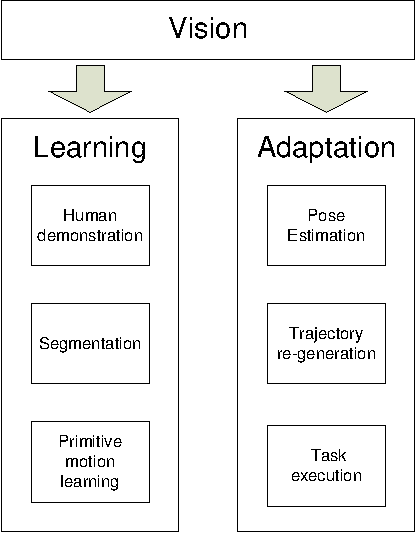
\includegraphics[width=5cm]{./fig/overview.pdf}
\caption{\scriptsize{System overview of bimanual sewing robot}}

\label{fig:overview}
}
\end{figure}

\begin{enumerate}
\item{1}: Needle pose re-detection
\item{2}: Trajectory adaptation
\end{enumerate}

\begin{figure}
\centering
{
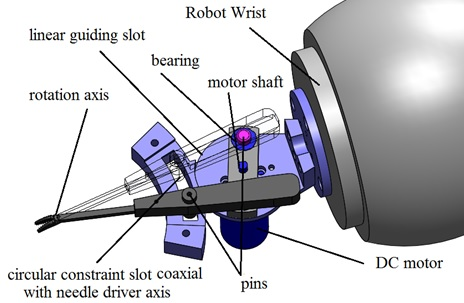
\includegraphics[width=5cm]{./fig/needledriver.jpg}
\caption{\scriptsize{Motorized needle driver}}

\label{fig:overview}
}
\end{figure}

